\documentclass{exam-zh}
\usepackage{siunitx}
\usepackage{graphicx}
\usepackage{draftwatermark}
\usepackage{twemojis}

% 用 Twemoji 显示彩色 emoji（字体本身不含 💤 字形）。
% twemoji 的 zzz 对应 U+1F4A4，1.5em 大小与正文基本齐平。
\newcommand{\zzzemoji}{\raisebox{-0.3em}{\twemoji[height=1.5em]{zzz}}}

\SetWatermarkText{工试群版权所有，仅供学习，严禁商用}           % 设置水印内容
\SetWatermarkLightness{0.9}             % 设置水印透明度 0-1
\SetWatermarkScale{0.3}                   % 设置水印大小 0-1


\examsetup{
  page/size=a4paper,
  paren/show-paren=true,
  paren/show-answer=true,
  fillin/show-answer=false,
  solution/show-solution=show-stay,
  solution/label-indentation=false,
  page/foot-content={试题第;页（共;页）}
}

\everymath{\displaystyle}

\graphicspath{{figures/}{2026/figures/}}

\title{上海交通大学2026年平台预分专业能力测试考试}

\subject{数学和逻辑}



\begin{document}

% \information{
%   姓名\underline{\hspace{6em}},
%   座位号\underline{\hspace{15em}}
% }
% \warning{（在此卷上答题无效）}

% \secret

\maketitle

本试卷共 60 题。全卷满分 100 分。考试用时 120 分钟。


\begin{notice}
  \item 上海交通大学工科试验班26群（1027107274）版权所有，禁止商用
  \item 制作人员：方天{\CJKfontspec{华文宋体}宬}（策划/整理/排版）、铁镐镐（整理）、Lucifinil、muqi、羊、陈自由、心归漫天、AltoliZy、炜-0211、Ayasesaki、
万、浮生、独燕成春\_Claire、Texas、栊翠庵下的雪、自扰庸墨、唐牢娅、ZOMBIEIEIEIE、HCOOMA、ZEM、\zzzemoji{}、qmgqmgqmg、WFstars、纪念日、
栩栩如生、墨染秋池、Riiiiva、ZZY、lkl45d、Hoshio、himilktea（万梓皓）、自由之风劲吹、林地受害者欧穆、6、栗子、沨
  \item 本卷是回忆版，疏漏之处请见谅；第 52 题原始素材缺失，欢迎补充
\end{notice}



\section{%
  数学部分：共 30 小题，1 到 10 题每小题 1 分，11 到 30 题每小题 2 分。
}

% 1
\begin{question}
直线 $a$ 在平面 $\beta$ 上，对于直线$l$, $l\perp a$ 是 $l\perp\beta$ 的 \paren[]
\begin{choices}
  \item 充分非必要条件
  \item 必要非充分条件
  \item 充要条件
  \item 非充分非必要条件
\end{choices}
\end{question}

% 2
\begin{question}
已知 $(1+2i)z=3-4i$，$i$ 是虚数单位，求 $|z|=$ \paren[]
\begin{choices}
  \item $\sqrt{5}$
  \item $1$
  \item $\sqrt{3}$
  \item $5$
\end{choices}
\end{question}

% 3
\begin{question}
将 $2$ 个 $0$ 和 $4$ 个 $1$ 随机排列成 $1$ 行，那么 $2$ 个 $0$ 相邻的概率为 \paren[]
\begin{choices}
  \item $\dfrac{1}{3}$
  \item $\dfrac{2}{5}$
  \item $\dfrac{1}{5}$
  \item $\dfrac{1}{2}$
\end{choices}
\end{question}

% 4
\begin{question}
$f(x)=\cos\left(2x+\dfrac{\pi}{6}\right)$ 的函数图像向左移动 $\varphi>0$ 个单位，得到的新图像关于原点对称，则 $\varphi$ 的最小值为 \paren[]
\begin{choices}
  \item $\dfrac{\pi}{12}$
  \item $\dfrac{\pi}{6}$
  \item $\dfrac{\pi}{3}$
  \item $\dfrac{\pi}{2}$
\end{choices}
\end{question}

% 5
\begin{question}
若多项式 $x^4+ax^2+bx+c$ 能被 $(x-1)^3$ 整除，则 $3a+2b+c=$ \paren[]
\begin{choices}
  \item $5$
  \item $3$
  \item $-5$
  \item $-3$
\end{choices}
\end{question}

% 6
\begin{question}
$\left(2x-\dfrac{1}{x}\right)^6$ 的展开式中常数项为 \paren[]
\begin{choices}
  \item $80$
  \item $160$
  \item $-80$
  \item $-160$
\end{choices}
\end{question}

% 7
\begin{question}
平行四边形 $\mathrm{ABCD}$，$\mathrm{AB}=6$，$\mathrm{AD}=4$，$\angle \mathrm{BAD}=60^\circ$，$\overrightarrow{\mathrm{DE}}=\overrightarrow{\mathrm{EC}}$，$\overrightarrow{\mathrm{AB}}=2\overrightarrow{\mathrm{BF}}$，求 $\overrightarrow{\mathrm{AE}}\cdot\overrightarrow{\mathrm{EF}}=$ \paren[]
\begin{choices}
  \item $7$
  \item $8$
  \item $9$
  \item $10$
\end{choices}
\end{question}

% 8
\begin{question}
已知 $x,y\in\mathbb{R}$，$x+3y=6$，求 $\min\left(2^x+8^y\right)=$ \paren[]
\begin{choices}
  \item $32$
  \item $12$
  \item $16$
  \item $8$
\end{choices}
\end{question}

% 9
\begin{question}
已知 $x=a(t-\sin t)$，$y=a(1-\cos t)$，对于 $f(x)$ 的函数图像，下列说法正确的是 \paren[]
\begin{choices}
  \item 关于原点对称
  \item 关于 $x=\pi$ 对称
  \item 周期为 $2a\pi$
  \item 周期为 $2\pi$
\end{choices}
\end{question}

% 10
\begin{question}
双曲线 $\dfrac{x^2}{a^2}-\dfrac{y^2}{b^2}=1\ (a>0,b>0)$，$F_1,F_2$ 是双曲线的左、右焦点，点 $\mathrm{E}$ 在双曲线左支上，$\angle F_1EF_2=\dfrac{2}{3}\pi$，$2|\mathrm{EF}_1|=|\mathrm{EF}_2|$，该双曲线的离心率是 \paren[]
\begin{choices}
  \item $\sqrt{3}$
  \item $3$
  \item $\sqrt{7}$
  \item $\sqrt{5}$
\end{choices}
\end{question}

% 11
\begin{question}
$f(x)=x^3-3x$ 在 $[a,b]$ 上的值域为 $[-2,2]$，则 $b-a$ 的最小值为 \paren[]
\begin{choices}
  \item $1$
  \item $\sqrt{3}$
  \item $2$
  \item $3$
\end{choices}
\end{question}

% 12
\begin{question}
将 $8$ 个相同的小球放入 $3$ 个不同的盒子中，要求每个盒子小球不超过 $4$ 个，放法种数共有 \paren[]
\begin{choices}
  \item $15$
  \item $18$
  \item $24$
  \item $27$
\end{choices}
\end{question}

% 13
\begin{question}
椭圆 $\dfrac{x^2}{a^2}+\dfrac{y^2}{b^2}=1\ (a>b>0)$ 的离心率为 $e=\dfrac{\sqrt{3}}{2}$，且过点 $\left(\sqrt{3},0\right)$，则该椭圆的焦距为 \paren[]
\begin{choices}
  \item $\sqrt{3}$
  \item $3$
  \item $2\sqrt{3}$
  \item $6$
\end{choices}
\end{question}

% 14
\begin{question}
若 $p$ 和 $2p+1$ 都是奇素数，则 $5p-1$ \paren[]
\begin{choices}
  \item 必然是素数
  \item 必然是合数
  \item 可能是合数可能是素数
  \item 以上都不对
\end{choices}
\end{question}

% 15
\begin{question}
一个二项展开式中有相邻三项的二项式系数为 $1:2:3$，则该二项式的次数为 \paren[]
\begin{choices}
  \item $11$
  \item $12$
  \item $13$
  \item $14$
\end{choices}
\end{question}

% 16
\begin{question}
在一场 $135$ 个人参加的宴会上，人们相互握手，他们每三个人中至少有两个人握过手，其中握手次数最多的一位是甲，则甲至少握手多少次？\paren[]
\begin{choices}
  \item $65$
  \item $66$
  \item $67$
  \item $68$
\end{choices}
\end{question}

% 17
\begin{question}
从 $1$ 到 $30$ 这 $30$ 个不同的正整数中任意选取三个不同的数，使这三个数的和能被 $3$ 整除，则满足条件的选取方法共有多少种？\paren[]
\begin{choices}
  \item $1360$
  \item $1200$
  \item $1400$
  \item $1160$
\end{choices}
\end{question}

% 18
\begin{question}
在正四棱锥 $P-ABCD$ 中，所有侧面均为边长为 $1$ 的正三角形。设 $M$ 为 $AB$ 的中点，$N$ 为 $BC$ 的中点，则异面直线 $MN$ 与 $PC$ 之间的距离为 \paren[]
\begin{choices}
  \item $\dfrac{\sqrt{2}}{4}$
  \item $\dfrac{\sqrt{3}}{4}$
  \item $\dfrac{\sqrt{2}}{3}$
  \item $\dfrac{\sqrt{3}}{3}$
\end{choices}
\end{question}

% 19
\begin{question}
$f(x)=\log_2(x^2-3x+2)$，则 $f(x)<1$ 时 $x$ 的范围是 \paren[]
\begin{choices}
  \item $(0,3)$
  \item $(0,1)$
  \item $(0,1)\cup(2,3)$
  \item $(-\infty,1)\cup(2,3)$
\end{choices}
\end{question}

% 20
\begin{question}
椭圆 $C$：$\dfrac{x^2}{a^2}+\dfrac{y^2}{b^2}=1\ (a>b>0)$，$N$ 是右顶点，$M$ 是右焦点，$|MN|=4$，直线 $y=kx$ 交椭圆于 $P,Q$，$P$ 在第二象限，$l_{\mathrm{PM}}$ 平分线段 $\mathrm{QN}$，求 $a^2+b^2=$ \paren[]
\begin{choices}
  \item $68$
  \item $49$
  \item $40$
  \item $14$
\end{choices}
\end{question}

% 21
\begin{question}
已知抛物线 $y^2=2px\ (p>0)$，一条直线交抛物线于 $A,B$ 两点，焦点为 $F$，$|\mathrm{FA}|=2|\mathrm{FB}|$，且 $FA\perp FB$，请问 $AB$ 斜率为 \paren[]
\begin{choices}
  \item $\pm 1$
  \item $\pm\sqrt{2}$
  \item $\pm\sqrt{3}$
  \item $\pm 2$
\end{choices}
\end{question}

% 22
\begin{question}
函数列 $F_k(x)$ 满足递推关系：$F_0(x)=x$，$F_{n+1}(x)=[F_n(x)]^2-1\ (n=0,1,2,3,\cdots)$，则方程 $F_4(x)=0$ 的相异实根个数为 \paren[]
\begin{choices}
  \item $5$
  \item $4$
  \item $8$
  \item $7$
\end{choices}
\end{question}

% 23
\begin{question}
一位运动员在训练中打靶 $8$ 次，得分分别为 $9.7$，$9.8$，$9.5$，$9.3$，$9.4$，$9.9$，$9.6$，$10.0$，其中 $m\%$ 分位数为 $x$，在他的打靶成绩中任选一个，大于 $x$ 的概率是 $25\%$，那么 $m$ 不能是 \paren[]
\begin{choices}
  \item $65$
  \item $70$
  \item $75$
  \item $80$
\end{choices}
\end{question}

% 24
\begin{question}
$\mathbb{R}$ 上的奇函数 $f(x)$ 满足 $f\left(\dfrac{3}{2}+x\right)=f(-x)$，$f(1)=-3$。数列 $\{a_n\}$ 满足 $a_1=-1$，$S_n=2a_n+n$，$S_n$ 为前 $n$ 项和，则 $f(a_5)+f(a_6)=$ \paren[]
\begin{choices}
  \item $2$
  \item $3$
  \item $-2$
  \item $-3$
\end{choices}
\end{question}

% 25
\begin{question}
一组数据 $x_1,x_2,\cdots,x_n$ 的平均值为 $4$，方差为 $2$，求数据 $2x_1+1,2x_2+1,\cdots,2x_n+1$ 的平均值和方差分别为 \paren[]
\begin{choices}
  \item $8$ 和 $4$
  \item $8$ 和 $8$
  \item $9$ 和 $4$
  \item $9$ 和 $8$
\end{choices}
\end{question}

% 26
\begin{question}
$MN$ 与 $BC$ 交于 $BC$ 的中点 $O$，$\overrightarrow{\mathrm{AB}}=m\overrightarrow{\mathrm{AM}}$，$\overrightarrow{\mathrm{AC}}=n\overrightarrow{\mathrm{AN}}$，求 $\dfrac{2}{m}+\dfrac{1}{n}$ 的最小值为 \paren[]
\begin{choices}
  \item $3$
  \item $\dfrac{3}{2}\sqrt{2}$
  \item $\dfrac{3}{2}+\sqrt{2}$
  \item $\dfrac{5}{2}$
\end{choices}
\begin{center}
  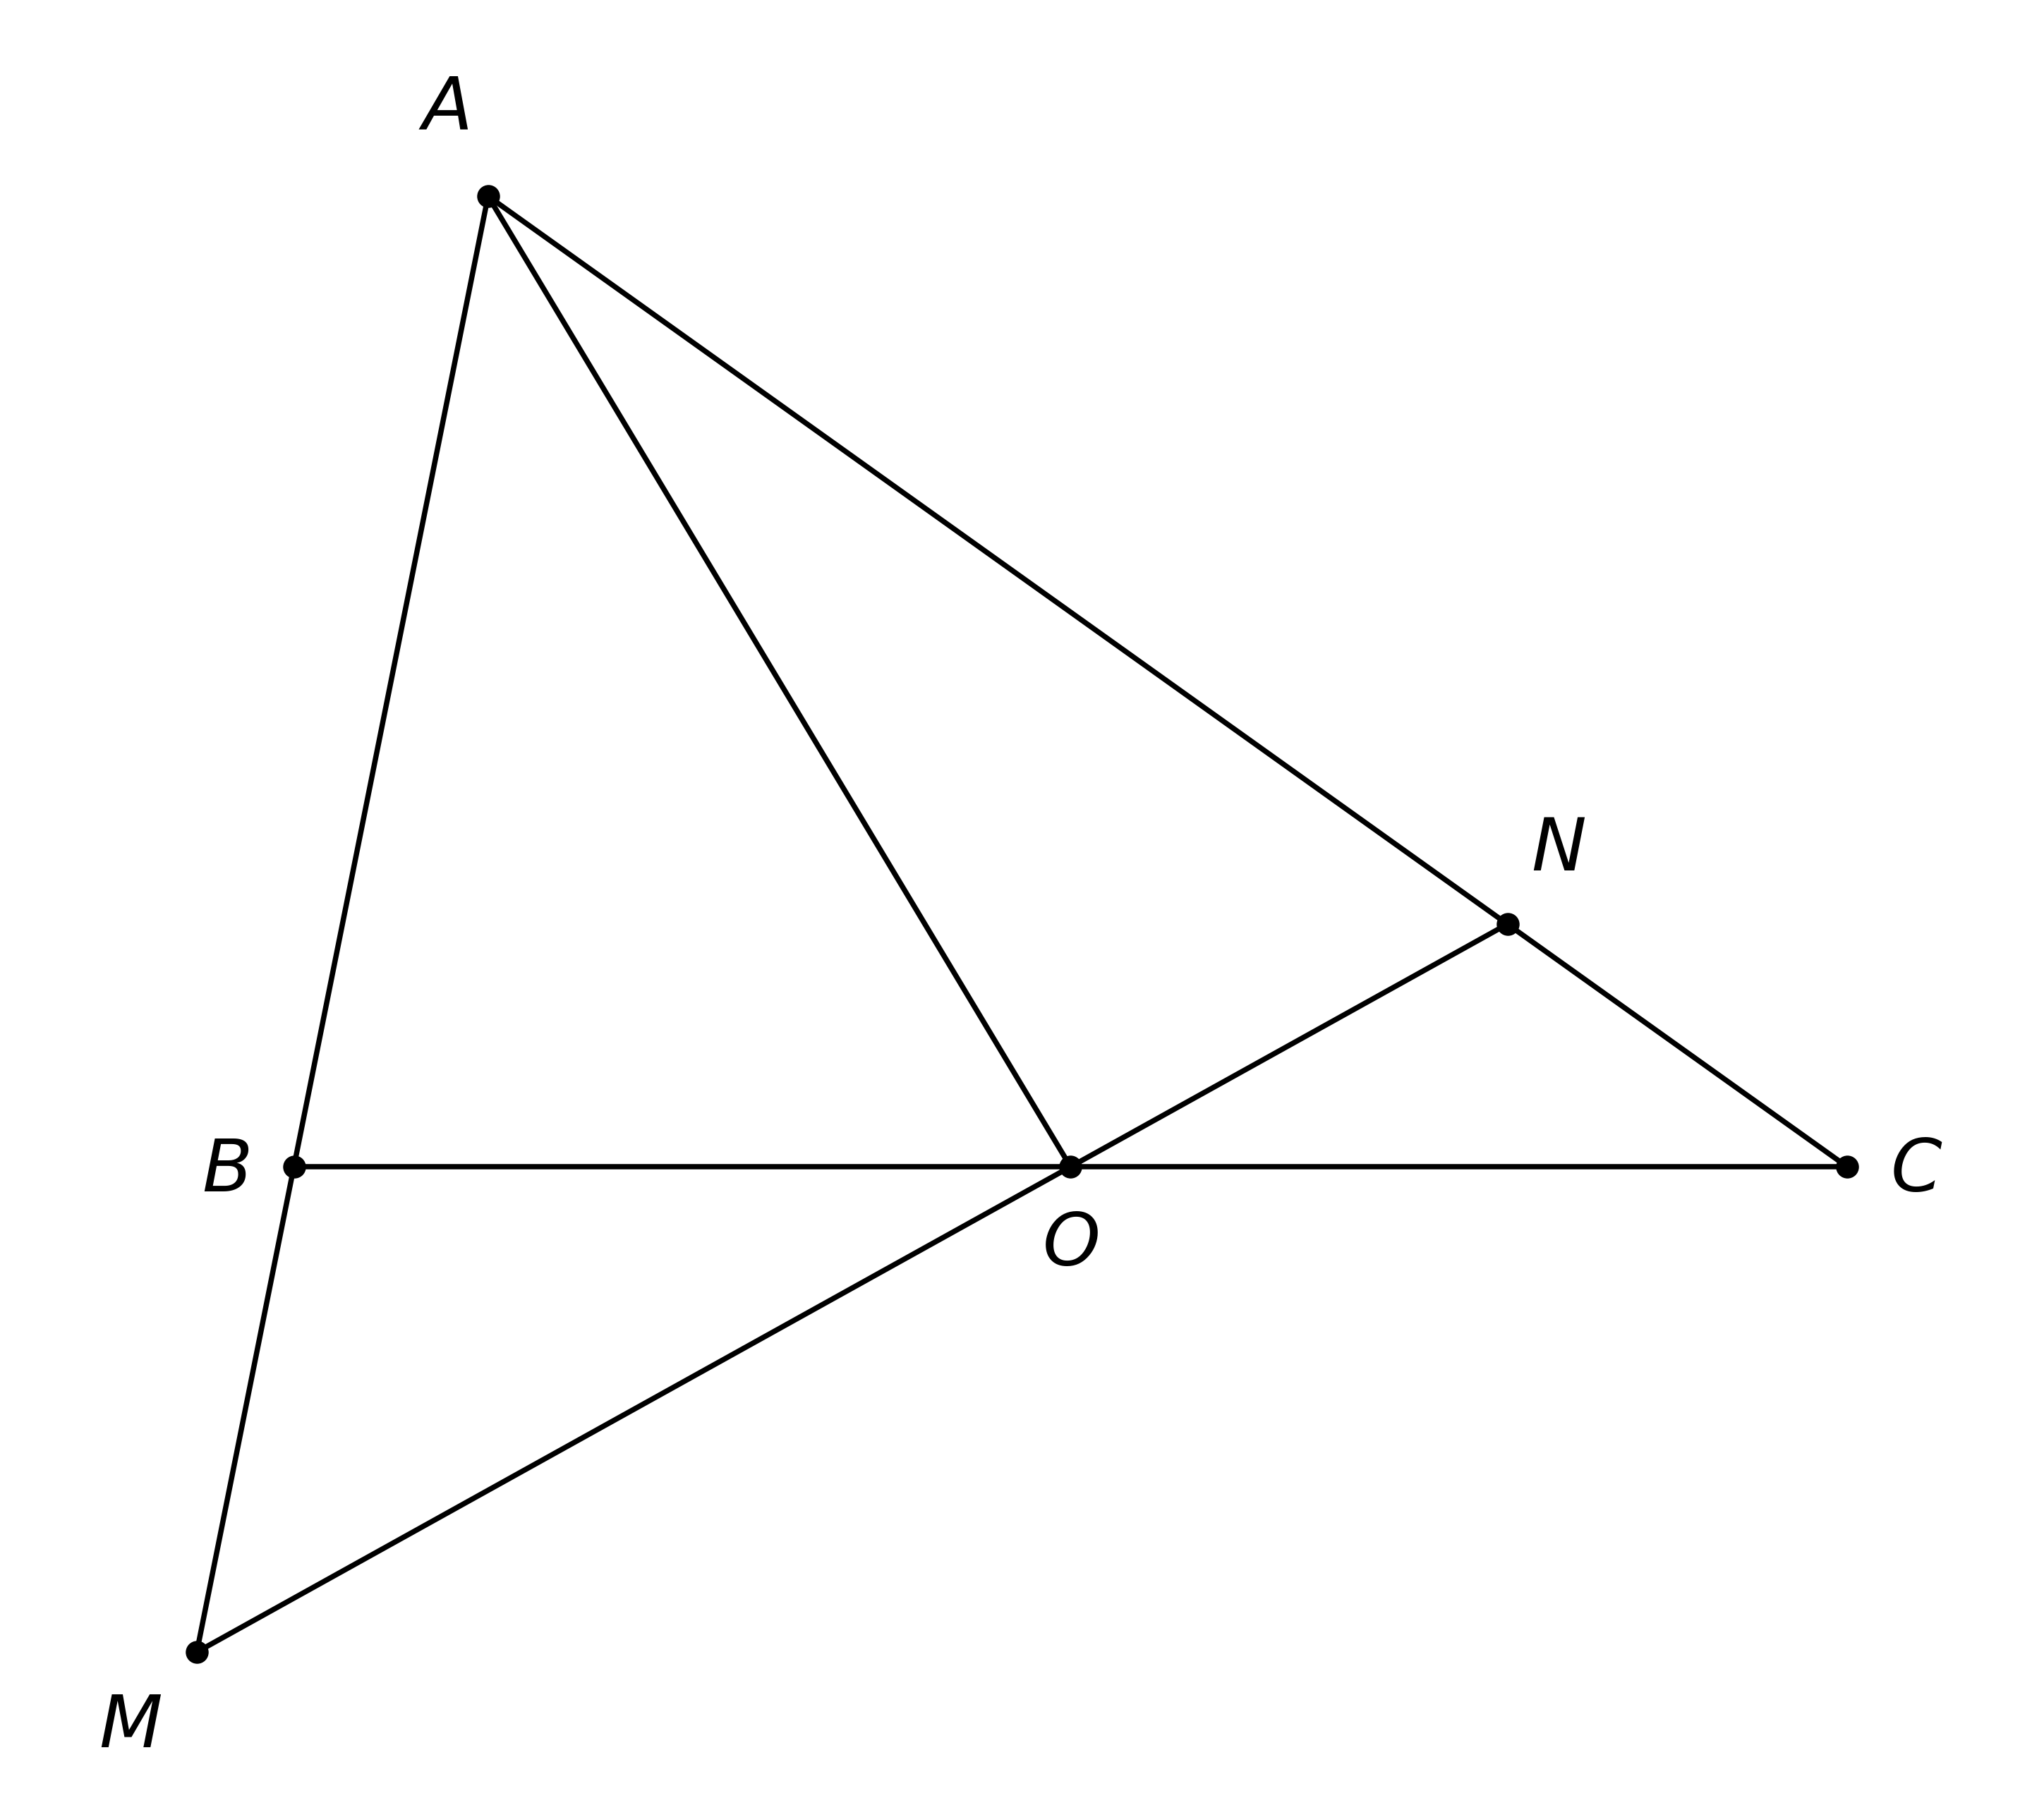
\includegraphics[width=0.55\textwidth]{math-26.png}
\end{center}
\end{question}

% 27
\begin{question}
$f(x)=2\sin x+\cos x-\sqrt{5}x$，$a=f(\lg 2)$，$b=f(\ln 3)$，$c=f((-1)^0)$，则 \paren[]
\begin{choices}
  \item $a>b>c$
  \item $a>c>b$
  \item $b>c>a$
  \item $c>a>b$
\end{choices}
\end{question}

% 28（题图较大，单独换页，避免图与题目分离）
\begin{question}
直三棱柱 $ABC-A_1B_1C_1$ 中，若 $BC=2AB=2$，$AA_1=AC=\sqrt{3}$，$M$ 是 $B_1C_1$ 的中点，过 $AM$ 作这个三棱柱的截面，当截面与平面 $ABC$ 所成的锐二面角最小时，这个截面的面积为 \paren[]
\begin{choices}
  \item $2$
  \item $\dfrac{\sqrt{15}}{2}$
  \item $\dfrac{5\sqrt{3}}{6}$
  \item $\sqrt{3}$
\end{choices}
\end{question}

% 29
\begin{question}
斐波那契数列是连接自然现象和数理逻辑的经典模型，已知该数列满足 $F_1=F_2=1$，$F_{n+2}=F_{n+1}+F_n\ (n\ge1)$，那么 $F_{2026}$ 除以 $8$ 所得的余数为 \paren[]
\begin{choices}
  \item $1$
  \item $3$
  \item $5$
  \item $7$
\end{choices}
\end{question}

% 30
\begin{question}
为描述两点间沿坐标系绕行的最短距离，研究路径算法与坐标选址等现实问题，给出直角距离的定义，记点 $\mathrm{P}$ 到点 $\mathrm{Q}$ 的直角距离为 $d(\mathrm{P},\mathrm{Q})=|x_{\mathrm{P}}-x_{\mathrm{Q}}|+|y_{\mathrm{P}}-y_{\mathrm{Q}}|$。关于直角距离，有以下两项说法：

① 原点 $\mathrm{O}$ 到直线 $x-y+1=0$ 上一点的直角距离最小为 $\dfrac{\sqrt{2}}{2}$。

② 记 $\mathrm{P},\mathrm{Q}$ 两点间直线距离为 $|\mathrm{PQ}|$，那么恒有 $|\mathrm{PQ}|\ge\dfrac{\sqrt{2}}{2}d(\mathrm{P},\mathrm{Q})$。

对于这两项说法，\paren[]
\begin{choices}
  \item ①正确
  \item ②正确
  \item ①②均正确
  \item ①②均不正确
\end{choices}
\end{question}


\section{%
  逻辑部分：共 30 小题，31 到 40 题每小题 1 分，41 到 60 题每小题 2 分。
}

% 31
\begin{question}
根据男婴出生率，甲和乙展开了辩论。

甲：人口统计发现一条规律：在新生婴儿中，男婴的出生率总是摆动于 $22/43$ 这个数值，而不是 $1/2$。

乙：不对，许多资料都表明，多数国家和地区，例如俄罗斯、日本、美国、德国，以及我国的台湾地区都是女人比男人多。可见，认为男婴出生率总在 $22/43$ 上下波动是不成立的。

试分析甲乙的对话，指出下列选项中哪一个能说明甲或乙的逻辑错误？\paren[]
\begin{choices}
  \item 甲所说的统计规律并不存在
  \item 甲的统计调查不符合科学
  \item 乙混淆了概念
  \item 乙的资料不可信
\end{choices}
\end{question}

% 32
\begin{question}
“试点综合症”的问题现在屡见不鲜。每出台一项改革措施，先进行试点，积累经验后再推广，这种以点带面的工作方法本来是人们经常采用的。但现在许多项目中出现了“一试点就成功，一推广就失败”的怪现象。以下最可能是造成上述现象的原因的是 \paren[]
\begin{choices}
  \item 在选择试点单位时，一般选择比较好的单位。
  \item 社会一般会十分关注试点的进行与推广。
  \item 在试点过程中，领导往往比较重视，各方面的问题解决得快。
  \item 试点尽管成功，但许多企业外部的政策、市场环境却并不相同。
\end{choices}
\end{question}

% 33
\begin{question}
挤出效应是指市政府通过扩大财政支出、增加贷款来刺激市场经济，进而抑制或减少了私人部门（企业和家庭）的财政消费的现象。根据上述定义，下列最能体现挤出效应的是 \paren[]
\begin{choices}
  \item 增加投入建设低空经济飞行产业园，促进民营飞行器企业加入
  \item 通过增加专项贷款来建设高铁，从而刺激投资，进而抑制、减少民营企业的融资
  \item 提高进口关税，增加本土产业份额，减少进口产品占比
  \item 增加对新能源汽车消费者的补贴，抑制传统燃油汽车的消费
\end{choices}
\end{question}

% 34
\begin{question}
某超级城市的建设部决定要在五年内建成覆盖全市的低空交通网络，实现市内通勤时间缩短至原来的 $50\%$。建设部这样做隐含了什么前提？\paren[]
\begin{choices}
  \item 五年内低空载具的运载成本会下降至可接受的范围
  \item 市民不会因为低空载具的噪音等问题进行大规模抗议
  \item 现有电池能量密度及航空器技术，足以支撑低空载具实现高峰频次的安全飞行
  \item 其他大城市也在同步推进低空交通网络的建设
\end{choices}
\end{question}

% 35
\begin{question}
企业只有拥有自主可控的底层算法，且拥有海量的高质量训练数据，才能生成超大规模语言模型。据此，下列选项为真的是 \paren[]
\begin{choices}
  \item 若某企业拥有超大规模语言模型，则一定拥有自主可控的底层算法。
  \item 若某企业没有超大规模语言模型，一定是因为没有海量的高质量训练数据。
  \item 若某企业拥有海量高质量数据和自主可控的底层算法，一定可以生成超大规模语言模型。
  \item 若某企业拥有自主可控的底层算法，但没有海量的高质量数据，也有可能生成超大规模语言模型。
\end{choices}
\end{question}

% 36
\begin{question}
根据德摩根定律，工程师认为：并非（该电子元件既达到 $3\,\mathrm{nm}$ 又降低 $50\%$ 能耗）。据此，以下为真的是 \paren[]
\begin{choices}
  \item 该电子元件达到 $3\,\mathrm{nm}$，或者降低了 $50\%$ 能耗
  \item 该电子元件没有达到 $3\,\mathrm{nm}$，也没有降低 $50\%$ 能耗
  \item 该电子元件没达到 $3\,\mathrm{nm}$，那么就要降低 $50\%$ 能耗
  \item 该电子元件没有达到 $3\,\mathrm{nm}$，或者没有降低 $50\%$ 能耗
\end{choices}
\end{question}

% 37
\begin{question}
某重点中学最近一项调查表明，该校高中生对踢足球有着特殊偏好，而且远远超过了其他球类，调查同时发现经常踢足球的学生学习成绩比不经常踢足球的学生好。由此可见，经常踢足球能够提高学生的学习成绩。以下哪项最能削弱上述结论？\paren[]
\begin{choices}
  \item 该校经学生家长同意订立了一条规定：只有学习成绩排名在年级前 $30\%$ 的高中生才能够经常踢足球
  \item 经常踢足球能够锻炼身体，进而保持旺盛的学习精力
  \item 经常踢足球耽误了学习时间
  \item 科学研究并没有证明，经常踢足球有助于智力开发
\end{choices}
\end{question}

% 38
\begin{question}
稻草人谬误是指在论辩中歪曲、夸大或虚构对方主张，将其替换为更易攻击的版本并加以反驳的谬误。下列说法最符合稻草人谬误的是 \paren[]
\begin{choices}
  \item 甲：“我认为城市应该增加自行车道数量来鼓励绿色出行。”乙：“你是要禁止所有私家车出行，让人类文明重回农耕时代吗？这根本行不通！”
  \item 甲：“这批新药的临床样本量还不够。”乙：“如果这批新药不能及时上市，会有更多的病人得不到救治。”
  \item 甲：“我认为应该控制人工智能的研发速度来评估风险。”乙：“人工智能是核心竞争力，这会导致国家落后。”
  \item 甲：“这部手机太贵了。”乙：“一分钱一分货，高品质的产品自然是高成本。”
\end{choices}
\end{question}

% 39
\begin{question}
诉诸权威是指在论证过程中，仅仅以某人在某一领域的权威地位或身份作为论据——尤其当其权威身份与主张方向不符时——而不考虑其言论本身是否具有合理性或事实依据的逻辑谬误。根据上述定义，下列选项中属于诉诸权威的是 \paren[]
\begin{choices}
  \item 某物理学家运用广义相对论，通过严密的数学推导预测了黑洞的存在
  \item 某数学家通过严密的逻辑论证，成功证明了数论中的一道世界级难题
  \item 国际上数百名传染病学专家联合发表倡议书，呼吁公众要注意预防传染病
  \item 某知名影视明星为某款保健品代言，称该产品能包治百病并推荐大众购买
\end{choices}
\end{question}

% 40
\begin{question}
二分谬误，又称假两难推理，是逻辑学中的一种论证谬误，属于分散注意谬误。其特征是将复杂问题简化为两个看似互斥的选项，并错误地声称已穷尽所有可能性，而实际上忽略了其他合理选择。以下犯了二分谬误的是 \paren[]
\begin{choices}
  \item 一个人参加考试，要么通过，要么不通过。
  \item 一个正整数，要么是奇数，要么是偶数。
  \item 一个人，要么支持我的方案，要么反对我的方案，没有第三种可能，反对我的都是我的敌人。
  \item 抛一枚硬币，要么正面朝上，要么反面朝上。（忽略正立的可能）
\end{choices}
\end{question}

% 41
\begin{question}
关于某国家级量子计算实验室的科研人员组成，有如下四个断定：
\begin{enumerate}
  \item 该实验室所有科研人员都具有博士学位；
  \item 该实验室有些科研人员没有博士学位；
  \item 该实验室负责人张教授具有博士学位；
  \item 该实验室有些科研人员具有博士学位。
\end{enumerate}
已知上述 $4$ 个断定之中恰有 $2$ 个为真，$2$ 个为假。据此，可以推断出 \paren[]
\begin{choices}
  \item 张教授具有博士学位
  \item 张教授没有博士学位
  \item 所有科研人员都没有博士学位
  \item 无法判断张教授有没有博士学位
\end{choices}
\end{question}

% 42
\begin{question}
某地对企业开展低空经济活动作出如下规定：
\begin{enumerate}
  \item 如果一家企业想要从事低空经济活动，那么它必须取得低空运营许可证，并购买高额第三者责任保险。
  \item 如果一家企业想要取得低空运营许可证，那么它必须拥有国家级重点实验室。
  \item 甲公司能够从事低空经济活动。
\end{enumerate}
根据上述条件，可以必然推出以下哪一项？\paren[]
\begin{choices}
  \item 甲公司拥有国家级重点实验室。
  \item 如果一家企业拥有国家级重点实验室，那么它就一定能够取得低空运营许可证。
  \item 如果一家企业没有购买高额第三者责任保险，那么它仍有可能从事低空经济活动。
  \item 如果一家企业取得了低空运营许可证，那么它就一定购买了高额第三者责任保险。
\end{choices}
\end{question}

% 43
\begin{question}
关于我国某重型运载火箭发射，四位专家分别进行了评论：

甲：只要一二级火箭分离成功，就可以进入轨道。

乙：一二级火箭分离成功，但没进入轨道。

丙：要么一二级火箭没有分离成功，要么没进入轨道。

丁：火箭进入了轨道。

已知四位专家中只有一位专家的评论为真，那么下列选项正确的是 \paren[]
\begin{choices}
  \item 甲对，火箭进入了轨道
  \item 乙对，火箭一二级分离成功
  \item 丙对，火箭没有进入轨道
  \item 丁对，火箭进入了轨道
\end{choices}
\end{question}

% 44
\begin{question}
多国科研团队围绕 AGI 通用人工智能是否需要设立全球暂停研发的协定展开研讨。某国科学家发表观点：
如果不设定暂停研发的协定，相关配套安全治理体系就难以跟上技术迭代速度，会引发难以管控的安全风险；
而一旦设定全球暂停协定，由于各国科研发展节奏、政策执行力度不同，暂停周期会出现明显差异，这会造成本国在技术赛道上落后于人。
于是要么引发不可控的安全风险，要么本国技术陷入落后局面。该科学家得出结论所隐含的前提是 \paren[]
\begin{choices}
  \item 设定暂停协定能够彻底解决 AGI 带来的安全风险
  \item AGI 带来的安全风险比本国技术落后的危害更大
  \item 要么选择设定暂停协定，要么选择不设定暂停协定
  \item 世界上所有国家都会严格遵守统一的暂停期约定
\end{choices}
\end{question}

% 45
\begin{question}
在信息高速发展的时代，短视频、有声听书、内容梗概等轻量化阅读形式不断涌现。当代年轻人获取信息的渠道日趋多元，
不再局限于完整研读整本原著，碎片化速读而非按部就班地一本一本看书成为很多人的阅读习惯。但专家提出，倘若你打算读一本书，至少要读完它的前 $30$ 页。
下列哪个选项如果为真，可以最好支持专家的主张？\paren[]
\begin{choices}
  \item 学习本就是枯燥的，学习就是学习，娱乐就是娱乐，从来不存在所谓“娱乐化学习”一说。
  \item 有些人拿到一本书后，能够津津有味地一直读下去，并不会感到枯燥乏味。
  \item 一本书的前 $30$ 页通常是对全书概念术语的引入，跨过这个门槛是顺利读完全书的关键。
  \item 很多令人读起来开心、频频点头的读物看似有趣，实际上是读者已知知识的无效堆叠，对于学习新事物毫无益处。
\end{choices}
\end{question}

% 46
\begin{question}
某新能源电池实验室研发出一款固态电解质材料，该电池在零下 $30$ 摄氏度的极寒条件下放电容量损耗不到 $85\%$，且充放电 $1500$ 次后电量缩减不到 $10\%$，据此某研究人员认为该电池已具备完全替代传统电解液电池并在寒冷地区大面积商业化的技术条件。下列哪个选项如果为真，可以最好支持该研究人员的结论？\paren[]
\begin{choices}
  \item 该固体电解质使用的原料储备丰富，且成本不超过传统电解液的 $60\%$
  \item 传统电解液电池在零下 $20$ 度时的电容损耗超过 $35\%$
  \item 各大主流车企均在着手部署新型固体电解质的研发管线
  \item 该固体电解质电池在高温条件下的安全性能测试正在稳步进行
\end{choices}
\end{question}

% 47
\begin{question}
科研人员在实验室条件下证实：某种细菌可分泌 PET 降解酶，高效分解 PET 塑料。据此专家断言：将该菌种投入垃圾填埋场，就能够彻底解决 PET 塑料带来的白色污染问题。以下哪个选项最能支持该专家的观点？\paren[]
\begin{choices}
  \item 这种酶即使在工业酸碱环境下依然能保持高催化活性
  \item PET 只占白色垃圾的 $10\%$ 左右
  \item PET 可以填埋燃烧
  \item PET 降解酶分解 PET 塑料效率很高
\end{choices}
\end{question}

% 48
\begin{question}
某国开展能源转型，太阳能和风能等可再生能源的装机容量提升了 $80\%$。然而同期该国碳排放总量却没有下降，反而比三年前高了 $5\%$。若以下哪项为真，最可以解释这种看似矛盾的现象？\paren[]
\begin{choices}
  \item 可再生能源发电装置的运输和制造过程中会产生少量碳排放
  \item 为推广可再生能源，国家为消费者提供了财政补贴和大量政策优惠
  \item 公众对可再生能源的接受度较高，纷纷安装了家用光伏板
  \item 可再生能源的发电具有间歇性，为保证用电安全，政府增设了火电站作为基荷电源的补燃发电量
\end{choices}
\end{question}

% 49
\begin{question}
目前，新兴半导体产业迅速发展，某公司半导体产业利润率增长 $18\%$，相关先进制造及技术材料（$\le 28\,\mathrm{nm}$）购进率增长 $70\%$，与此同时，AI 产业硬件需求增长，相关高带宽内存（HBM）利用与开发率持续保持在 $100\%$。由此可推断出 \paren[]
\begin{choices}
  \item 相关先进制造及技术材料（$\ge 28\,\mathrm{nm}$）的产业已全面萎缩
  \item AI 浪潮推动了新兴半导体产业相关先进制造及技术材料产业的发展
  \item 新兴半导体产业将完全占领市场
  \item 传统产业已经（或将要）失去生存发展的土壤
\end{choices}
\end{question}

% 50
\begin{question}
随着大模型广泛落地应用，AI“幻觉”问题逐渐受到大众关注。AI 幻觉是指大模型在生成文本时，出现虚构事实、张冠李戴、编造引用等输出虚假信息的现象，严重制约了 AI 回答的可信度。某专家对此提出观点：AI 产生幻觉，根源是预训练阶段所使用的训练数据集存在事实错误、信息缺失等纰漏。因此，搭建纯净数据库、使用高质量内容做训练素材，是训练可靠高效 AI、缓解幻觉问题的核心。以下哪一项如果为真，最能削弱该专家的观点？\paren[]
\begin{choices}
  \item 即使使用经过多层人工校验、完全无事实错误的高质量纯净数据集进行训练，大模型依然会产生幻觉
  \item 引入 RAG 检索增强技术，让模型在回答时调取外部权威真实资料，能够显著降低大模型幻觉的发生概率
  \item 某研究发现，大模型的幻觉问题是模型概率生成机制本身带来的固有特性，与数据没有必然关联
  \item 人类在回忆久远记忆时，也会出现类似的“幻觉”，与 AI 的“幻觉”表现形式极其类似
\end{choices}
\end{question}

% 51
\begin{question}
有人认为：传统国家电网类似于传统大型计算机，一旦遭受攻击，便可能面临全面瘫痪的危机；而智能微电网类似于分布式互联网，各个节点之间相互支持和连接，即使局部受损也能正常运行。因此，应当全面将国家电网改造成微智能电网，以彻底解决国家能源安全问题。以下哪项如果为真，最能够反驳上述观点？\paren[]
\begin{choices}
  \item 分布式互联网在遭受大型攻击时，仍然会有局部瘫痪。
  \item 智能微电网的电能传输与分布式互联网的连接与路由有着本质区别。
  \item 微智能电网的建设与后期维护成本远高于传统大型电网。
  \item 目前许多国家都在尝试将大型电网与智能微电网结合运行。
\end{choices}
\end{question}

% 52
\begin{question}
（本题原始回忆素材缺失）
\end{question}

% 53
\begin{question}
甲：工业机器人投入生产会替代大量重复性劳动岗位，造成结构性失业问题，因此应当对引入机器人的企业征收机器人税。

乙：参考多国自动化生产历史实践，虽然自动化会淘汰部分低端岗位，但也会创造附加值更高的新岗位，从长远看能够提升社会整体福利，征收机器人税反而会阻碍产业进步。

甲乙二人争论的焦点是什么？\paren[]
\begin{choices}
  \item 当下将机器人投入生产是否成熟
  \item 引入机器人的整体影响是正面还是负面
  \item 政府是否应当对企业征收机器人税
  \item 重复性劳动岗位是否应被高附加值岗位取代
\end{choices}
\end{question}

% 54
\begin{question}
某文章宣称：“数据显示，在过去一年的交通事故中，驾驶新能源汽车发生事故的驾驶员，有 $80\%$ 驾龄在三年以下，而驾驶传统燃油车的驾驶员，驾龄在三年以下的仅占 $30\%$。这充分说明了新能源汽车的操作复杂性远高于燃油车，更容易导致新手驾驶员发生交通事故。”以下哪项最能指出上述文章在利用数据进行推理时的逻辑陷阱？\paren[]
\begin{choices}
  \item 未考虑不同驾驶员在购买保险时的赔付比例差异。
  \item 未给出新能源汽车和传统汽车具体的交通事故总绝对数量。
  \item 未说明这些交通事故是由汽车机械故障还是驾驶员主观失误导致的。
  \item 忽略了在近年来新能源汽车的新买家中，低驾龄新手驾驶员所占比例本来就比燃油车高这一基数背景。
\end{choices}
\end{question}

% 55
\begin{question}
有四个外观相同的小球，编号分别为甲乙丙丁，它们的重量可能不同。用一个天平称重，将甲和乙放在天平一侧，丙和丁放在另一侧，两侧基本相平；将乙和丁互换位置，甲和丁所在的一侧明显重于乙丙一侧；将甲、丙放在一侧，将乙放在另一侧，还没来得及放上丁，乙那一侧就明显重于甲丙一侧。问：四个小球从重到轻的顺序是？\paren[]
\begin{choices}
  \item 丁、乙、甲、丙
  \item 丁、乙、丙、甲
  \item 乙、甲、丁、丙
  \item 乙、丁、甲、丙
\end{choices}
\end{question}

% 56
\begin{question}
欧盟出台碳关税政策，要求进入欧盟市场的进口产品配套碳排放核算评估体系，依据商品生产环节的碳排放量征收对应关税。高碳排放企业的产品需要缴纳较高碳关税，会削弱该产品在欧盟市场的价格竞争力；低碳排放企业的产品适用较低碳关税，有助于这类产品进入欧盟市场。据此，可以推出 \paren[]
\begin{choices}
  \item 发展中国家出口到欧盟的商品，其贸易优势会因为这项政策而大大削弱
  \item 若政府搭建相关机制，监测并降低生产过程中的碳排放，将有利于其下企业扩大产品市场
  \item 在这项政策的评估体系下，产品碳排放数值达标能抵消商品本身质量短板带来的劣势
  \item 高碳排放企业的产品，若无法降低碳排放，将难以在全球其他海外市场维持原有市场份额
\end{choices}
\end{question}

% 57
\begin{question}
在一场关于“是否应当限制基因编辑技术在人类胚胎上的应用”的辩论赛中，反方辩手提出“支持基因编辑技术的人根本无视了人类基本的伦理道德，这些人企图通过基因改造制造所谓的超人阶级，使普通人类沦为劣等种姓，最终毁灭人类社会文明”。关于对反方辩手逻辑上的缺陷评析，正确的是 \paren[]
\begin{choices}
  \item 犯了“诉诸无知”的错误，没有证明基因编辑对人类的长期影响
  \item 犯了“循环论证”的错误，用结果证明前提
  \item 犯了“混淆概念”的错误，混淆了“基因编辑”和“基因改造”
  \item 犯了“稻草人谬误”和“滑坡谬误”的错误，歪曲支持者的观点并进行无理的极端灾难预测
\end{choices}
\end{question}

% 58
\begin{question}
五位朋友（A、B、C、D、E）坐在一排观影，座位编号从左到右依次为 $1$ 到 $5$，已知：
\begin{enumerate}
  \item A 坐在 C 的旁边；
  \item B 坐在 D 的正左侧；
  \item E 既不坐在 $1$ 号位，也不坐在 $5$ 号位；
  \item C 坐在 $4$ 号位。
\end{enumerate}
根据以上分析可知，B 坐在 \paren[]
\begin{choices}
  \item $1$ 号位
  \item $2$ 号位
  \item $3$ 号位
  \item $4$ 号位
\end{choices}
\end{question}

% 59
\begin{question}
某大学教授告诉学生，在人工智能技术高速发展的当下，人文社科类学生必须掌握数据分析能力，否则将会在未来的就业市场上失去竞争力。为使该教授的论述成立，必须添加的前提是 \paren[]
\begin{choices}
  \item 掌握数据分析能力的人文社科类学生更容易取得高薪工作
  \item 就业市场对于具有“人文素养＋数据分析”综合能力背景的人才需求量巨大
  \item 不掌握数据分析能力的人文社科类学生将无法应对未来要求综合能力的市场需求
  \item 人工智能完全取代了传统的人文社科研究方法
\end{choices}
\end{question}

% 60
\begin{question}
某科技公司主管称：“近期我们的员工工作时长增加了 $20\%$，而公司专利数量也提高了 $20\%$，这充分说明科技员工加班能提升公司的创新能力。”以下说法不能反驳其观点的是 \paren[]
\begin{choices}
  \item 强拉因果：强行将加班时长增加与专利数量上升这两个同时发生的事件进行联系
  \item 偷换概念：强行将该公司的专利数量和该公司创新能力相等价
  \item 单一归因：忽略了专利数量提高的其他因素，如长期投入的爆发或政策变化等
  \item 样本缺失：未考虑其他未增加工作时间但专利数量仍然上升的科技公司的存在
\end{choices}
\end{question}

\end{document}
